\section{Evaluation}

In this section, we present experimental evaluations\footnote{Benchmarking automation infrastructure sources: \url{https://github.com/vkutuev/matrix-benchmark}.} of the Brahma.FSharp platform, demonstrating its core capabilities on conventional (non-HPC) devices\footnote{This configuration is particularly relevant for business applications built on .NET.}. 
We assess Brahma.FSharp performance in two representative use cases, detailed in the following sections\footnote{
Respective code is available on GitHub: \url{https://github.com/gsvgit/ImageProcessing/tree/matrix_multiplication}.    
}.
\begin{enumerate}
\item The first one is an image convolution that demonstrates utilization of several GPU-s using F\# MailboxProcessor.
\item \textbf{Image convolution}: showcases smooth multi-GPU utilization through F\#'s MailboxProcessor for efficient tasks distribution.
\item \textbf{Matrix multiplication}: demonstrates creation of generic strongly statically typed kernels, utilization of local and private memory for performance optimization, and portability across different devices.
\end{enumerate}


\subsection{Image Convolution}

We implemented image convolution as a demonstration of multi-GPU utilization.
As established in~\cite{aleaGPUasync}, F\#'s native asynchronous programming model significantly simplifies the creation of complex nonlinear computational workflows combining GPU computations with CPU processing and I/O operations.
Our implementation leverages F\#'s MailboxProcessor, which Brahma.FSharp exposes as the primary interface for GPU communication.
The kernel is simply wrapped as illustrated in Listing~\ref{lst:img_conv}. 
For workload distribution, we developed a basic load balancer that dynamically routes each new image to the GPU agent with the fewest pending messages in its input queue.

\begin{listing}[h]
  \begin{minted}[linenos]{fsharp}
let imgProcessor filter (imgSaver: MailboxProcessor<_>) =
    MailboxProcessor.Start(fun inbox ->
        let rec loop ... = async { // Async message processing loop
            let! msg = inbox.Receive() // Load message
            match msg with
            | EOS ch -> // Handle end of stream
                imgSaver.PostAndReply EOS
                ch.Reply()
            | Img img -> // Handle image
                let filtered = filter img // Convolution
                imgSaver.Post (Img filtered)
                return! loop ... }// Got to next message
        loop ...)
  \end{minted}
  \caption{MailboxProcessor-based wrapper for kernel to make it easier to integrate it to complex workflow}
  \label{lst:img_conv}
\end{listing}

We evaluate this solution on a \textbf{Lenovo} platform with two GPUs: NVIDIA GeForce MX150 and Intel(R) UHD Graphics 620.
We assume all images are loaded into RAM and converted to grayscale. 
A typical sequence of filters is applied: 3 Gaussian blur operations ($5 \times 5$ kernel) followed by edge detection ($5 \times 5$ kernel).
420 images (1gb of data) was handled in 40 seconds with two GPUs, in 64 seconds using Nvidia GPU only, and in 97 seconds using Intel GPU only.
These results demonstrate that even a naive multi-GPU workflow can achieve up to 30\% speedup compared to using only the fastest single GPU (NVIDIA) in the system.

\subsection{Matrix Multiplication}

We evaluate a generic kernel parametrized by types and operations (see Listing~\ref{lst:mXm_kernels}), implemented in F\#.
Several basic optimizations, inspired by ``Tutorial: OpenCL SGEMM tuning for Kepler'' by Cedric Nugteren\footnote{``Tutorial: OpenCL SGEMM tuning for Kepler'': \url{https://cnugteren.github.io/tutorial/pages/page1.html}}, were applied.
Namely, we use tiling in local and private memory.
However, the current version supports only square matrices and square tiles.

\begin{figure}
  \begin{center}
  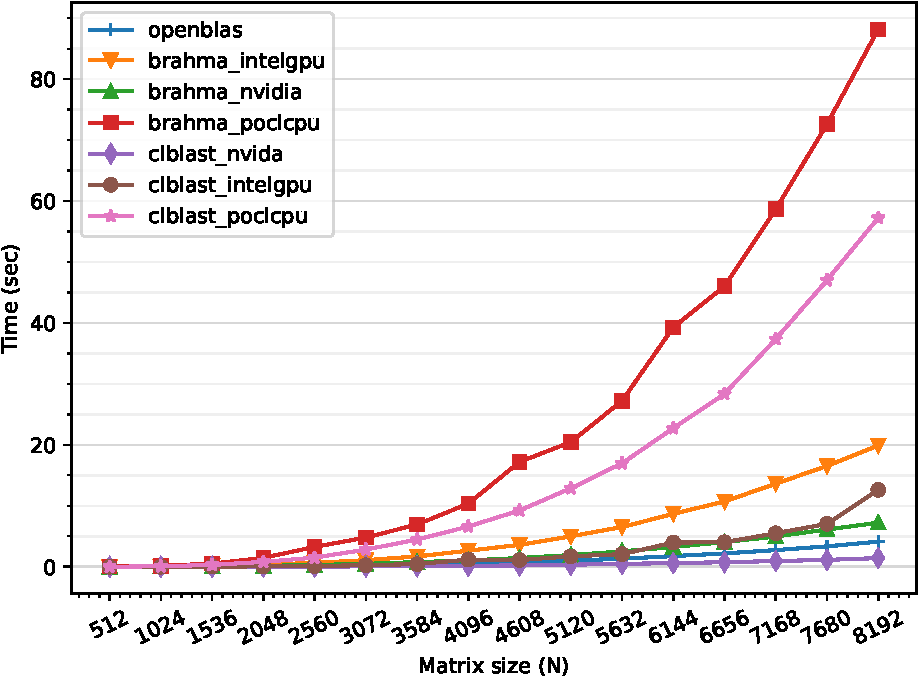
\includegraphics[width=0.45\textwidth]{../data/Lenovo-T480_crop.pdf}
  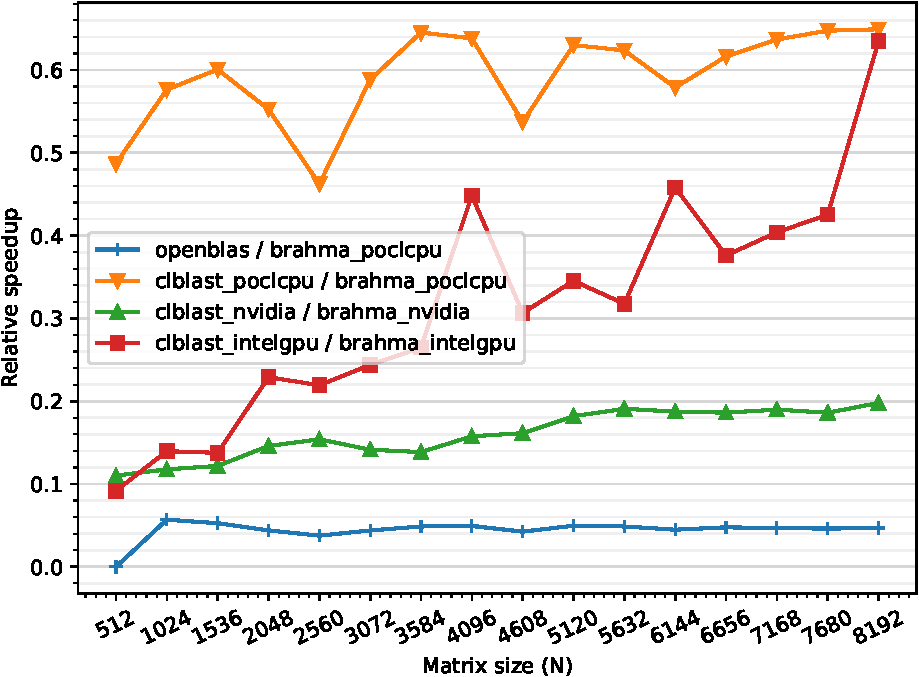
\includegraphics[width=0.45\textwidth]{../data/Lenovo-T480_rel_crop.pdf}\\
  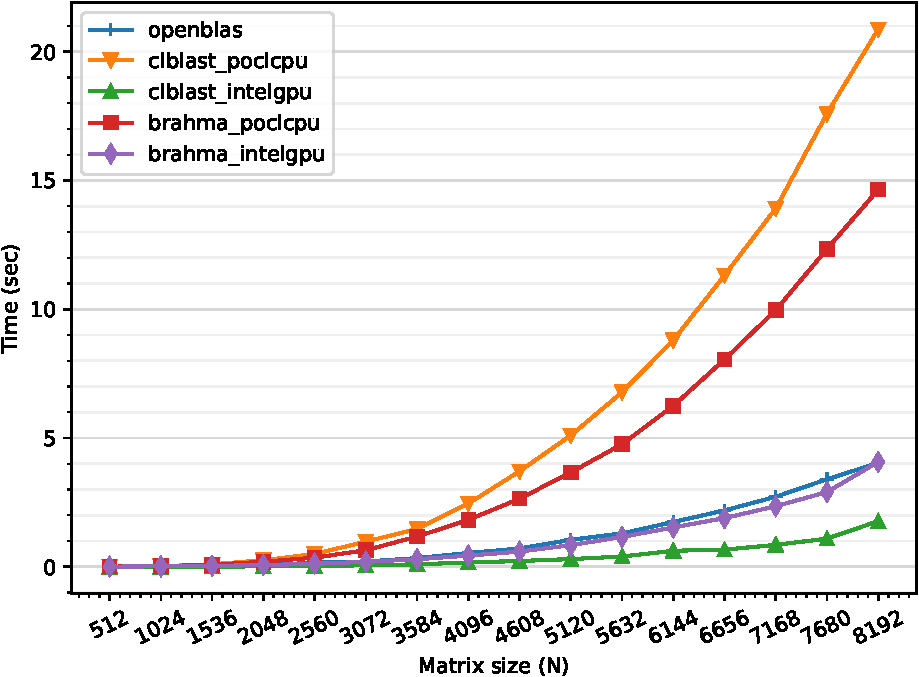
\includegraphics[width=0.45\textwidth]{../data/zenbook_iris_crop.pdf}
  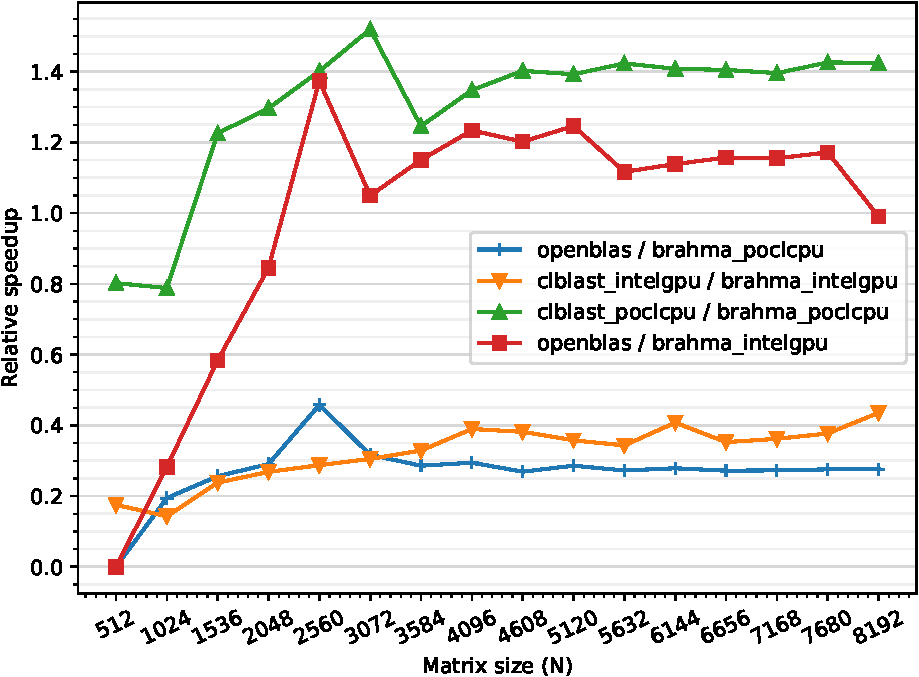
\includegraphics[width=0.45\textwidth]{../data/zenbook_iris_rel_crop.pdf}\\
  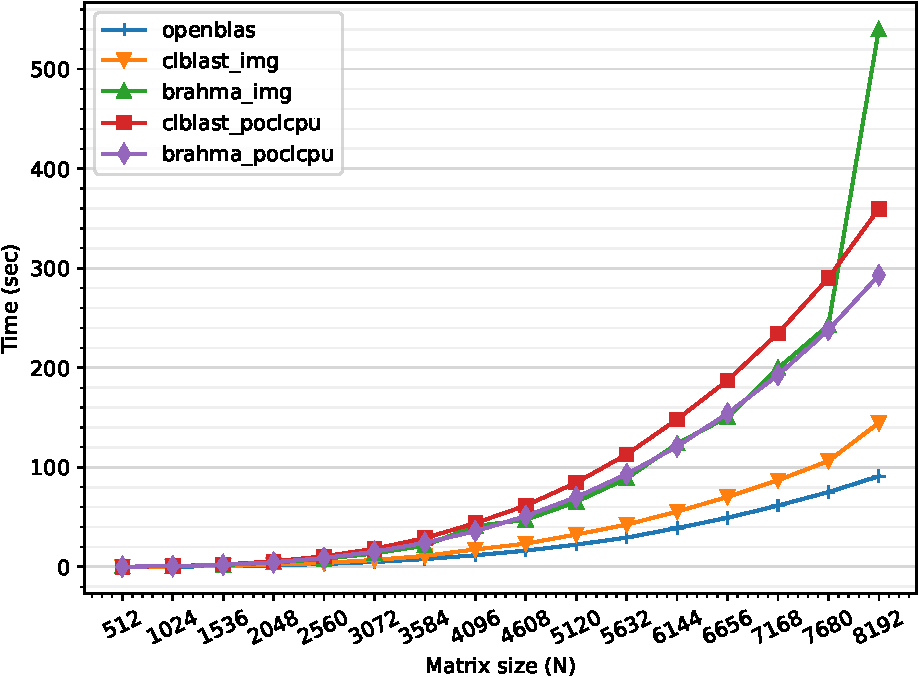
\includegraphics[width=0.45\textwidth]{../data/MILK-V_crop.pdf}
  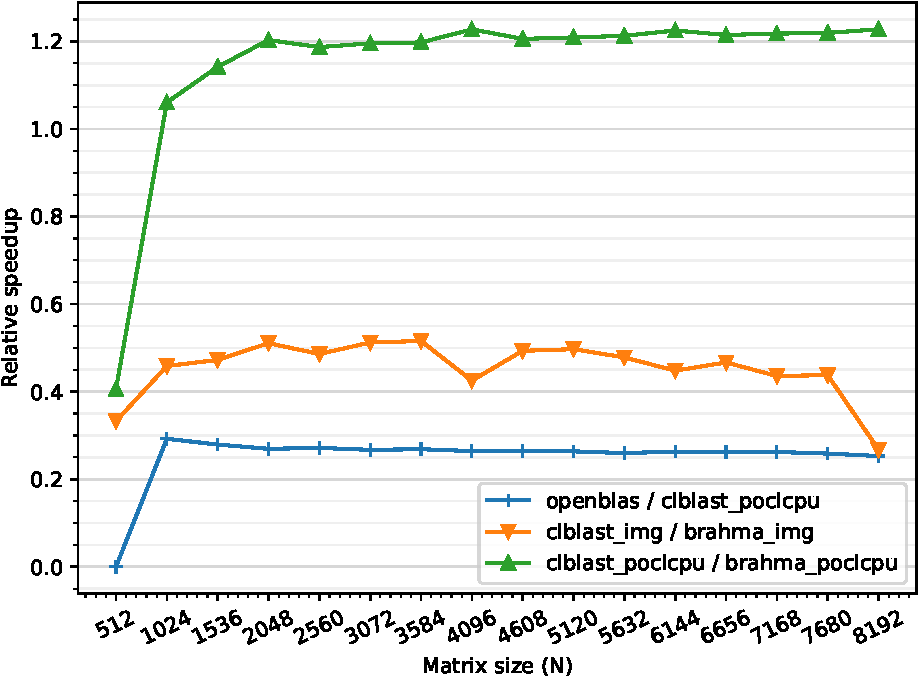
\includegraphics[width=0.45\textwidth]{../data/MILK-V_rel_crop.pdf}
  \end{center}
  \caption{Matrix multiplication performance: 1st row for \textbf{Lenovo}, 2nd for \textbf{Zen}, 3rd for \textbf{MILK-V}}
  \label{fig:mxm_perf}
\end{figure}

We selected two competitors for evaluation. 
The first is CLBlast\footnote{CLBlast source code: \url{https://github.com/CNugteren/CLBlast}}~\cite{10.1145/3204919.3204924}, a highly optimized OpenCL-based BLAS implementation tuned even for low-power mobile GPUs.
The second is OpenBLAS\footnote{OpenBLAS source code: \url{https://github.com/OpenMathLib/OpenBLAS}}, a highly optimized CPU-based BLAS implementation.
Additionally, we executed OpenCL-based solutions on CPUs using POCL~\cite{Jskelinen2014}.
All competitors were compiled and run with their default configurations.

We evaluate all competitors on several platforms listed below.
\begin{itemize}
  \item \textbf{Lenovo}: Intel Core i7-8550U CPU, NVIDIA GeForce MX150 and Intel UHD Graphics 620 GPUs.
  \item \textbf{Zen}: Intel Core i5-1340P CPU, Intel Iris Xe Graphics G7 80EUs GPU.
  \item \textbf{MILK-V}: SpacemiT M1 CPU, IMG BXE-2-32 GPU.
\end{itemize}

We generate random square matrices with elements of type \texttt{float32} and use the typical arithmetic semiring because our competitors do not provide generic kernels.
Time is measured as an average of 10 runs.
We measure time of client function execution, so it includes data transfer.
Results of the evaluation are represented in Figure~\ref{fig:mxm_perf}, where we show both time and relative speedup calculated as the ratio of corresponding average execution times.

First, we show that Brahma.FSharp allows one to create portable solutions.
While our kernel is not as optimized as the kernel from CLBlast, relative speedup analysis shows that there is a room for tuning: in many cases, the performance gap decreases with data size increase (\textbf{Lenovo} esp. Intel GPU; \textbf{Zen}).
However, in some cases the behavior is more complex: for \textbf{MILK-V}, our solution on CPU using POCL demonstrates better performance than CLBlast, but on the respective GPU the performance gap slightly increases with data size increase.

This behavior can be explained by differences in kernel tuning rather than by a Brahma.FSharp technology problem.
Thus, while it is unlikely possible to fully hide .NET overhead, it appears possible to minimize it to become comparable with competitors on large matrices. 
Following the methodology proposed in~\cite{10.1145/3204919.3204924}, we plan to support additional kernel parameters enabling more precise tuning of performance-critical aspects.